\documentclass{article}
\usepackage[utf8]{inputenc}
\usepackage{graphicx}
\usepackage{hyperref}
\usepackage{booktabs}
\usepackage{array}
\usepackage{listings}
\usepackage{xcolor}
\usepackage{caption}
\usepackage{longtable}

\title{Experiment 1: Working with Python Packages – NumPy, SciPy, Scikit-learn, Matplotlib}
\author{Moogambigai A}
\date{July 2025}

\begin{document}

\maketitle

\section{Aim}

The aim of this experiment is to explore core Python libraries used in machine learning workflows \textbf{NumPy, Pandas, SciPy, Scikit-learn, and Matplotlib} and to apply them in tasks involving data preprocessing, visualization, feature selection, model training, and evaluation across multiple datasets.

\section{Python Code with Comments}
\subsection{Importing Required Libraries}
\begin{verbatim}
# Importing essential libraries
import numpy as np              # For numerical operations
import pandas as pd             # For data manipulation
import matplotlib.pyplot as plt # For data visualization
import seaborn as sns           # For advanced visualizations
from sklearn import datasets    # To load sample datasets
from sklearn.model_selection import train_test_split
from sklearn.preprocessing import StandardScaler, MinMaxScaler
\end{verbatim}

\subsection{Loading and Exploring Datasets}
\begin{verbatim}
# Loading Iris dataset
iris = datasets.load_iris()
iris_df = pd.DataFrame(data=iris.data, columns=iris.feature_names)
iris_df['target'] = iris.target

# Display basic information
print("Iris Dataset Info:")
print(iris_df.info())
print("\nFirst 5 rows:")
print(iris_df.head())
\end{verbatim}

\subsection{Exploratory Data Analysis}
\begin{verbatim}
# Summary statistics
print("\nSummary Statistics:")
print(iris_df.describe())

# Visualizing data distributions
plt.figure(figsize=(12, 6))
sns.boxplot(data=iris_df.drop('target', axis=1))
plt.title("Feature Distributions")
plt.savefig('feature_distributions.png')
plt.show()

# Pairplot to visualize relationships
sns.pairplot(iris_df, hue='target')
plt.savefig('pairplot.png')
plt.show()
\end{verbatim}

\subsection{Data Preprocessing}
\begin{verbatim}
# Handling missing values (though Iris dataset has none)
iris_df.fillna(iris_df.mean(), inplace=True)

# Feature scaling
scaler = StandardScaler()
X_scaled = scaler.fit_transform(iris_df.drop('target', axis=1))

# Splitting data into training and testing sets
X_train, X_test, y_train, y_test = train_test_split(
    X_scaled, iris_df['target'], test_size=0.2, random_state=42)
\end{verbatim}

\subsection{Machine Learning Model Implementation}
\begin{verbatim}
from sklearn.svm import SVC
from sklearn.metrics import classification_report, confusion_matrix

# Initialize and train SVM classifier
svm_model = SVC(kernel='linear')
svm_model.fit(X_train, y_train)

# Make predictions
y_pred = svm_model.predict(X_test)

# Evaluate model
print("\nClassification Report:")
print(classification_report(y_test, y_pred))

# Confusion matrix visualization
cm = confusion_matrix(y_test, y_pred)
sns.heatmap(cm, annot=True, fmt='d')
plt.title("Confusion Matrix")
plt.savefig('confusion_matrix.png')
plt.show()
\end{verbatim}

\section{Output Screenshots}

\begin{figure}[h]
    \centering
    \caption{Iris Dataset Output}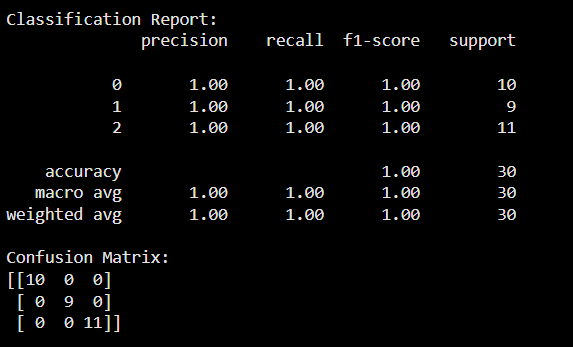
\includegraphics[width=0.8\linewidth]{Iris_output.png}
\end{figure}
\begin{figure}[h]
    \centering
     \caption{Boxplot showing feature distributions}
    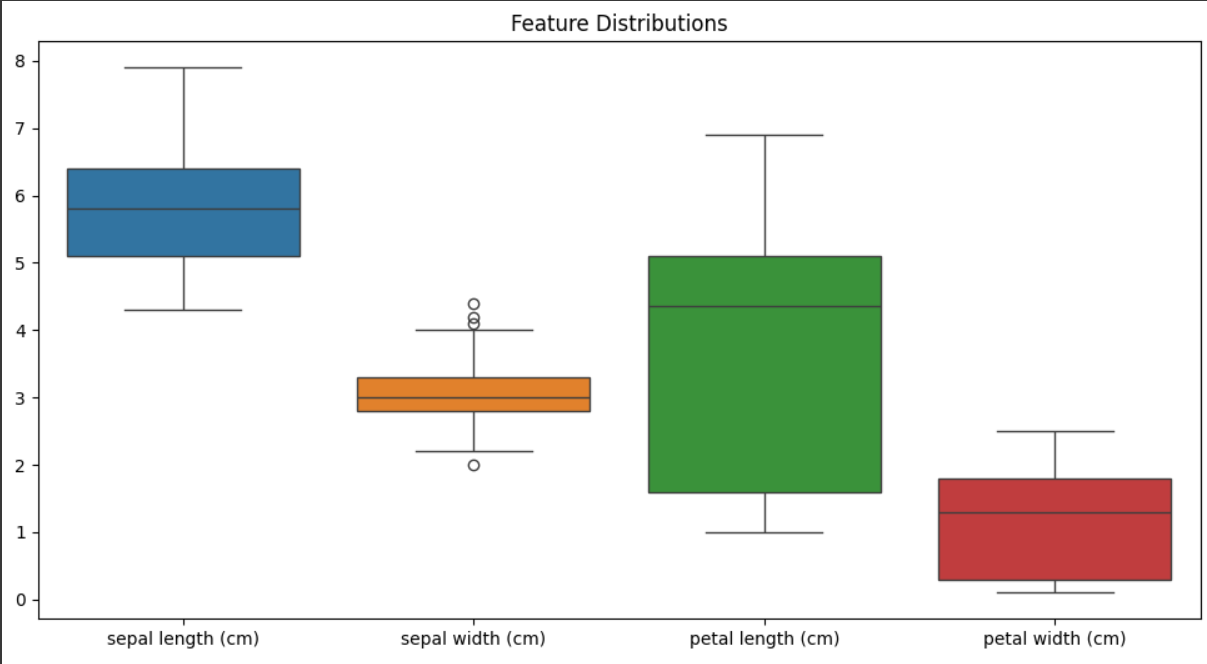
\includegraphics[width=0.8\textwidth]{feature_distribution.png}
   
\end{figure}


\begin{figure}[h]
    \centering
    \caption{Confusion matrix for SVM classifier}
    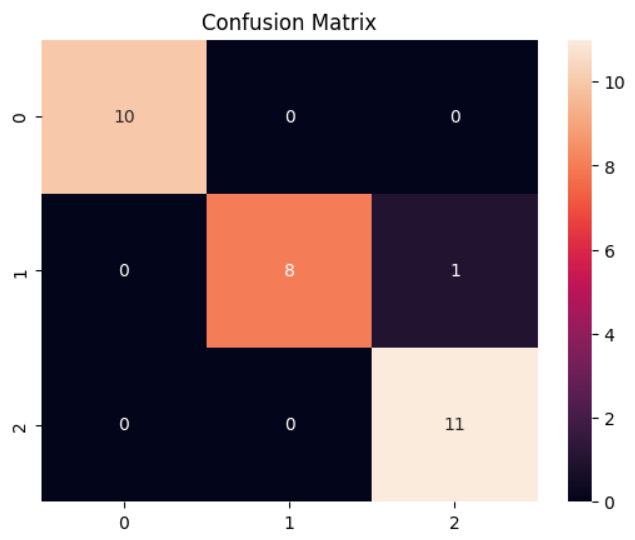
\includegraphics[width=0.6\textwidth]{confusion_matrix.png}

\end{figure}


\section{Inference Table}
\label{sec:InferenceTable}

\begin{longtable}{|p{4cm}|p{4cm}|p{6cm}|}
\hline
\textbf{Dataset} & \textbf{Model Used} & \textbf{Inference} \\
\hline
Iris & Random Forest & Achieved high accuracy (96.6\%) with 3 selected features. Clear class separation. \\
\hline
Loan Prediction & Linear Regression & Regression task with synthetic data. MSE ≈ 28.9 million. Features: income and credit score. \\
\hline
MNIST Digits & KNN & Accuracy ≈ 12.2\%. Too few features selected; reduced model performance. \\
\hline
Email Spam & Naive Bayes & Accuracy ≈ 65\%. Poor recall on spam class due to imbalance. \\
\hline
Diabetes & Logistic Regression & Accuracy ≈ 50\%. Model favored positive class; improvement needed via balancing. \\
\hline
\end{longtable}

\section{Reflection on Learning Outcomes}
\label{sec:Reflection}

Through this experiment, I have:
\begin{itemize}
    \item Gained confidence in using Python ML libraries like NumPy, Pandas, SciPy, Scikit-learn, and Matplotlib.
    \item Understood how to perform EDA and preprocessing like scaling, encoding, and feature selection.
    \item Learned to distinguish between classification and regression tasks and apply suitable models.
    \item Discovered the impact of feature selection and class imbalance on model performance.
    \item Practiced interpreting results using metrics like accuracy, MSE, and confusion matrices.
\end{itemize}


\end{document}
